\begin{figure}[H]
    \centering
    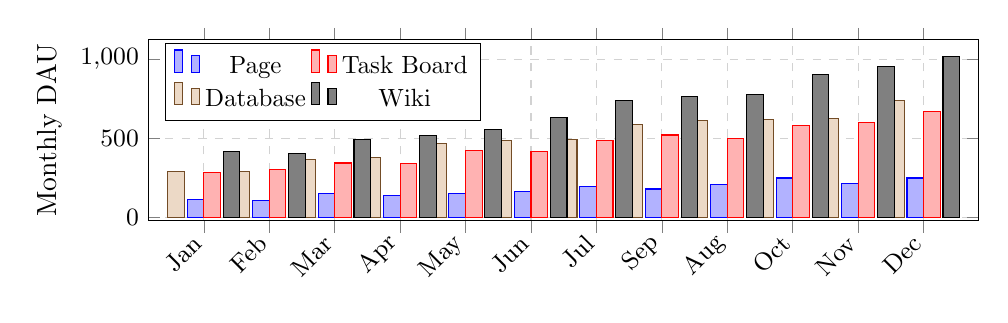
\begin{tikzpicture}
        \begin{axis}[
            width=\textwidth,
            height=0.32\textwidth,
            ybar,
            bar width=6pt,
            ylabel={Monthly DAU},
            ymin=0,
            ymax=1100,
            xmin=0.4,
            xmax=12.6,
            xtick={1,...,12},
            xticklabels={Jan,Feb,Mar,Apr,May,Jun,Jul,Sep,Aug,Oct,Nov,Dec},
            xticklabel style={rotate=45, anchor=east},
            tick label style={font=\small},
            legend style={at={(0.02,0.98)}, anchor=north west, nodes={scale=0.9, transform shape}},
            legend columns=2,
            grid=both,
            major grid style={dashed, gray!35},
            minor grid style={dotted, gray!20},
            enlargelimits=0.02,
            unbounded coords=discard
        ]
            \addplot+[bar shift=-3pt] coordinates {
                (1, 113) (2, 108) (3, 148) (4, 136) (5, 149) (6, 162)
                (7, 196) (8, 179) (9, 207) (10, 248) (11, 213) (12, 248)
            };
            \addplot+[bar shift=3pt] coordinates {
                (1, 281) (2, 303) (3, 343) (4, 339) (5, 420) (6, 413)
                (7, 487) (8, 520) (9, 499) (10, 582) (11, 600) (12, 668)
            };
            \addplot+[bar shift=-10pt] coordinates {
                (1, 289) (2, 292) (3, 367) (4, 377) (5, 469) (6, 488)
                (7, 489) (8, 586) (9, 612) (10, 617) (11, 626) (12, 736)
            };
            \addplot+[bar shift=10pt] coordinates {
                (1, 415) (2, 404) (3, 491) (4, 515) (5, 556) (6, 630)
                (7, 740) (8, 766) (9, 778) (10, 904) (11, 953) (12, 1014)
            };
            \legend{Page, Task Board, Database, Wiki}
        \end{axis}
    \end{tikzpicture}
    \caption{Seasonality by month across years (aggregated over 2024 - 2025).}
    \label{fig:kaq2-seasonality}
\end{figure}
